% !TeX root = ./IseliSchaller_Series02_ProgFuncLog.tex

\documentclass[12pt]{article}

\usepackage[
    a4paper,
    hmargin=2cm, vmargin=1.3cm,
    headheight=56.6pt, % as per the warning by fancyhdr
    headsep=10pt,
    includehead, includefoot
]{geometry}

\usepackage[french]{babel}
\usepackage[utf8x]{inputenc}
\usepackage[T1]{fontenc}

\usepackage{fancyhdr} % extensice control of page headers and footers
\usepackage{graphicx}
\usepackage{parskip} % add space between paragraphs and remove first line's indent
\usepackage[dvipsnames]{xcolor} % color the text for the color code: https://en.wikibooks.org/wiki/LaTeX/Colors
\usepackage[bottom]{footmisc} % to place footnotes to the bottom of the page
% \usepackage{amsmath} % provides math environments
\usepackage{ifthen} % provides \ifthenelse test
\usepackage{xifthen} % provides \isempty test
\usepackage{float} % improve the figure placement in the document
% \usepackage[acronym,nonumberlist,nogroupskip]{glossaries} % to handle acronyms
\usepackage{caption} % to change the style of the captions
\usepackage{listings}

% https://en.wikibooks.org/wiki/LaTeX/Source_Code_Listings -> Encoding problem
\lstset{literate=
  {á}{{\'a}}1 {é}{{\'e}}1 {í}{{\'i}}1 {ó}{{\'o}}1 {ú}{{\'u}}1
  {Á}{{\'A}}1 {É}{{\'E}}1 {Í}{{\'I}}1 {Ó}{{\'O}}1 {Ú}{{\'U}}1
  {à}{{\`a}}1 {è}{{\`e}}1 {ì}{{\`i}}1 {ò}{{\`o}}1 {ù}{{\`u}}1
  {À}{{\`A}}1 {È}{{\'E}}1 {Ì}{{\`I}}1 {Ò}{{\`O}}1 {Ù}{{\`U}}1
  {ä}{{\"a}}1 {ë}{{\"e}}1 {ï}{{\"i}}1 {ö}{{\"o}}1 {ü}{{\"u}}1
  {Ä}{{\"A}}1 {Ë}{{\"E}}1 {Ï}{{\"I}}1 {Ö}{{\"O}}1 {Ü}{{\"U}}1
  {â}{{\^a}}1 {ê}{{\^e}}1 {î}{{\^i}}1 {ô}{{\^o}}1 {û}{{\^u}}1
  {Â}{{\^A}}1 {Ê}{{\^E}}1 {Î}{{\^I}}1 {Ô}{{\^O}}1 {Û}{{\^U}}1
  {Ã}{{\~A}}1 {ã}{{\~a}}1 {Õ}{{\~O}}1 {õ}{{\~o}}1
  {œ}{{\oe}}1 {Œ}{{\OE}}1 {æ}{{\ae}}1 {Æ}{{\AE}}1 {ß}{{\ss}}1
  {ű}{{\H{u}}}1 {Ű}{{\H{U}}}1 {ő}{{\H{o}}}1 {Ő}{{\H{O}}}1
  {ç}{{\c c}}1 {Ç}{{\c C}}1 {ø}{{\o}}1 {å}{{\r a}}1 {Å}{{\r A}}1
  {€}{{\euro}}1 {£}{{\pounds}}1 {«}{{\guillemotleft}}1
  {»}{{\guillemotright}}1 {ñ}{{\~n}}1 {Ñ}{{\~N}}1 {¿}{{?`}}1
}
% https://tex.stackexchange.com/questions/82993/how-to-change-the-name-of-document-elements-like-figure-contents-bibliogr
\addto\captionsfrench{%
    % change the french name of tables etc.
    % \renewcommand{\tablename}{Tableau}
    \renewcommand{\lstlistingname}{Code}
    \renewcommand{\lstlistlistingname}{Liste de codes}
}
\definecolor{captioncolor}{rgb}{0.39, 0.33, 0.32} % caption color
\captionsetup[lstlisting]{font={color=captioncolor, small, tt}}
\DeclareCaptionFormat{listing}{\rule{\dimexpr\textwidth\relax}{0.4pt}\vskip1pt#1#2#3}
\captionsetup[lstlisting]{format=listing,singlelinecheck=false, margin=0pt, font={sf},labelsep=space,labelfont=bf}


\usepackage{hyperref}
\usepackage[inline]{enumitem} % allow to set some margin to list env's

% \usepackage{tikz}
% \usepackage{pgfplots}

% ---------------- SETUP HEADER & FOOTER ----------------------
\pagestyle{fancy}
% \fancyhf{} % sets both header and footer to nothing
% \renewcommand{\headrulewidth}{0pt} % remove headers bottom line


% Define variables
\makeatletter
\newcommand{\prof}[1]{\def\@prof{#1}}
\newcommand{\theprof}{\@ifundefined{@prof}{}{\\Prof.: \@prof}}
\newcommand{\student}[1]{\def\@student{#1}}
\newcommand{\thestudent}{\@ifundefined{@student}{}{\@student}}
\newcommand{\seriesnumber}[1]{\def\@seriesnumber{#1}}
\newcommand{\theseriesnumber}{\@ifundefined{@seriesnumber}{}{Série \@seriesnumber}}
\makeatother



\newcommand{\unilogo}[1][0.16\textwidth]{
\includegraphics[width=#1]{logo_uni}}

\newcommand*{\fullref}[1]{\hyperref[{#1}]{\autoref*{#1}} \textit{\nameref*{#1}}} % https://tex.stackexchange.com/a/121871
\newcommand*{\simpleref}[1]{\hyperref[{#1}]{{\autoref*{#1}}}}
\newcommand*{\namedref}[2]{\hyperref[{#1}]{\textit{#2}}}
\newcommand*{\visitedurl}[2]{\url{#1}\hspace{0.6em}(visited on #2)}
\newcommand*{\footnotelink}[2]{\footnote{\visitedurl{#1}{#2}}}
\newcommand*{\footnotetextlink}[2]{\footnotetext{\visitedurl{#1}{#2}}}

\newcommand*{\notice}[2][Notice]{
Remarque:
\begin{itemize}
    \vspace{-0.2cm}
    \item #2
\end{itemize}
}


\newcommand{\yellowInBlue}[1]{{\colorbox{blue!50}{\color{yellow}\textbf{#1}}}}

\newcommand*{\todo}[1]{
    \ifthenelse{\isempty{#1}}
        {\yellowInBlue{TODO}}
        {\yellowInBlue{TODO #1}} % else
}



\newcounter{question}
\newcommand{\questioncolor}{\color{CadetBlue}}
\def\newquestion#1{
    \refstepcounter{question}
    {
        \textbf{Exercice~\thequestion:}
        \questioncolor
        \emph{#1}
    }
}
\def\question#1{
    {
        \questioncolor
        \emph{#1}
    }
}


\setlist[description]{leftmargin=0.5cm,labelindent=0.5cm,parsep=0.4ex}


% \glsenablehyper
\hypersetup{
	colorlinks = true,
	% linkcolor = red,
	% menucolor = red,
	% filecolor = blue,
	% anchorcolor = green,
	% urlcolor = blue,
	allcolors = MidnightBlue,
	linkbordercolor = white
}


% \loadglsentries{glossary}
% \makeglossaries


\graphicspath{{assets/}}

\title{
    %\vspace{-2cm}
    \unilogo[0.3\textwidth]\\[0.9cm]
    Programmation fonctionnelle et Logique\\Haskell (Listes et récursivité)
}
\student{
    Yael Iseli \& A. Schaller\\
    \texttt{14-8215-24} \& \texttt{16-896-375}
}
\prof{Stéphane Le Peutrec}

\seriesnumber{2}
\author{\thestudent\theprof}

\lhead{\unilogo}
\rhead{\thestudent\\\theseriesnumber}

% \pgfplotsset{compat=newest}

% \usepackage[backend=bibtex, style=numeric, citestyle=numeric, sorting=none, backref, backrefstyle=none]{biblatex}
% use "biber report" command to generate

% \addbibresource{biblio.bib}


\raggedbottom % To avoid stretching the items to fill a page
% ---------------------- DOCUMENT ----------------------------
\begin{document}

\maketitle

%
%
% ---------------------------------
\section*{\theseriesnumber}

À travers les 4 exercices de la deuxième série,
nous devions réaliser plusieurs implémentations de fonction en utilisant ou non les motifs.

Comme plusieurs exemples sont donnés pour vérifier le comportement des fonctions,
nous étions intéressés de découvrir les solutions de tests disponibles dans l'écosystème \emph{Haskell}.

Rapidement, nous avons découvert \emph{hspec}\footnotelink{https://hspec.github.io/}{sept. 2020}.
Ses avantages sont:
\begin{itemize}
    \item il utilise une structure similaire à de nombreux aux frameworks de tests, tels que \emph{Jasmine}\footnotelink{https://jasmine.github.io/}{sept. 2020}, \emph{mocha}\footnotelink{https://mochajs.org/}{sept. 2020} et pleins d'autres.
    \item une prise en main qui parait rapide et simple avec \emph{cabal}\footnotelink{https://www.haskell.org/cabal/}{sept. 2020}.
\end{itemize}

Pour le dernier point, l'environnement du packages/librairies manager \emph{cabal} semble varier entre les systèmes.
Dans tous les cas, c'est une question d'un argument en plus un moins et de l'installation d'un, deux packages supplémentaires.

Dans tous les cas, nous sommes arrivé à pouvoir lancer les tests sur nos implémentations sans
devoir configurer un projet \emph{cabal} complet.

\begin{lstlisting}[language=bash,caption={Installation du package \emph{hspec}}]
cabal update && cabal install hspec
# dans certains cas, l'option --lib est nécessaire
# il est également possible de devoir installer 'QuickCheck'
# et 'base'
\end{lstlisting}

Finalement, nous pouvons exécuter nos tests que nous déclarons dans le \texttt{main} avec la commande \texttt{runhaskell}.
Le résultat obtenu dans le terminal est présenté dans la \simpleref{fig:tests_results}.

\begin{figure}[H]
    \center
    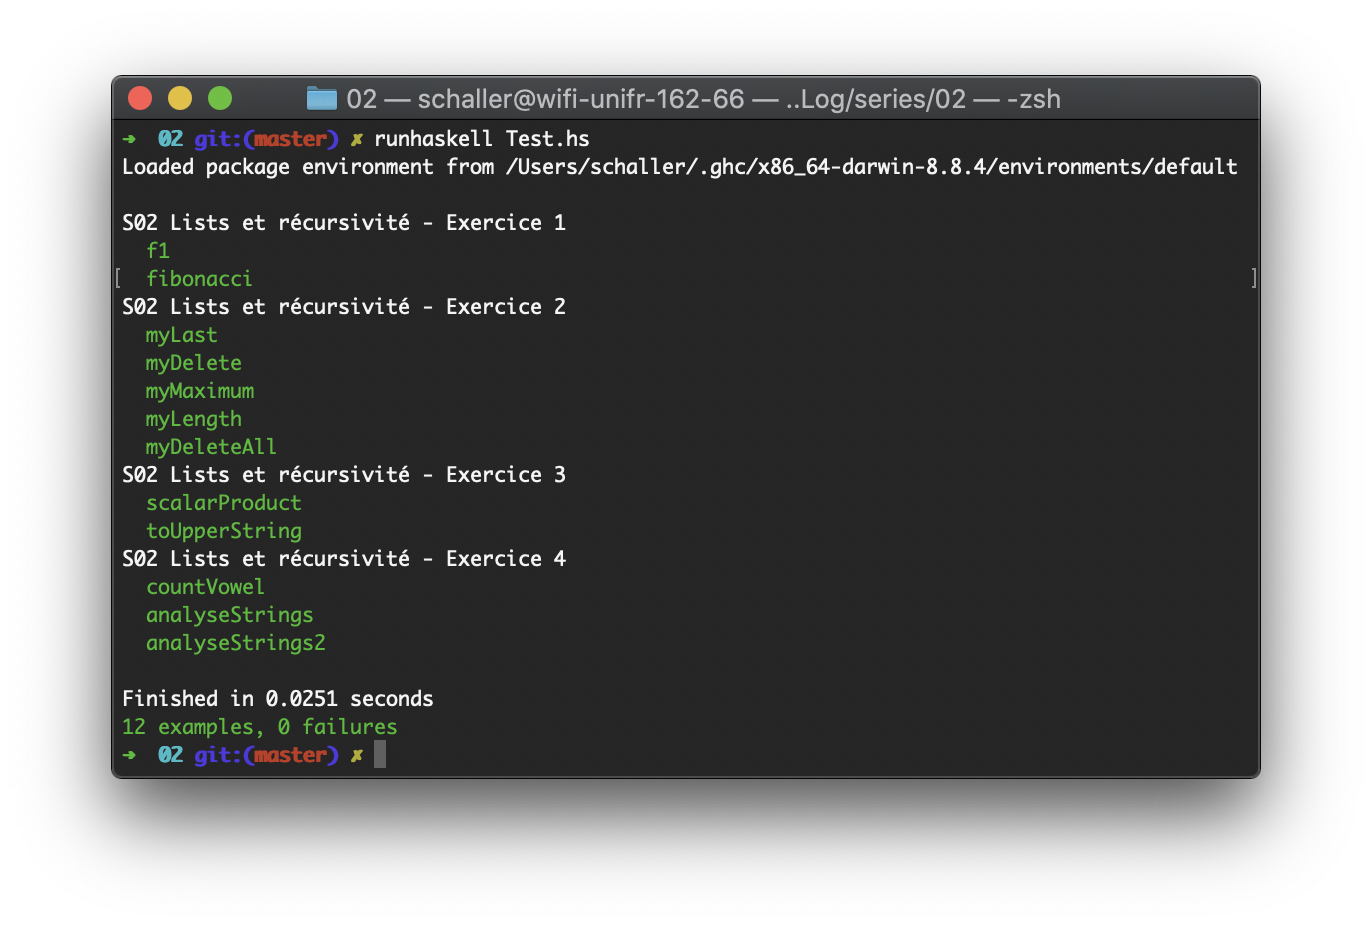
\includegraphics[width=0.9\textwidth]{series02/tests_results}
    \caption{\emph{hspec} tests results\label{fig:tests_results}}
\end{figure}

%
%
% ---------------------------------
\section*{Accès au code source}
Comme convenu, nous partageons le code source des séries sur notre \emph{Github} à l'adresse:
\begin{itemize}
    \item \url{https://github.com/schallerala/MSc-ProgFunLog}
\end{itemize}



% \notice{
%     Si le package \emph{hspec} ne suffit pas, il est possible qu'il soit nécessaire d'expliciter l'installation de \emph{QuickCheck} et \emph{base}
% }

%{
%\hypersetup{hidelinks}
%\printglossary % style=list2
%\printglossary[type=\acronymtype]
%}

% \section*{References}
% \printbibliography[heading=none]


%\section*{Appendix}
%\begin{itemize}
%   \item Exercise 1 \gls{Excel} spreadsheet\cite{s02-ex01-excel}
%\end{itemize}

\end{document}